\documentclass [11pt,twoside]{article}
\usepackage[utf8]{inputenc}
\usepackage[T1]{fontenc}

%Page margins, header and footer positions
\usepackage{geometry}
 \geometry{
 a4paper,
 total={210mm,297mm},
 left=25mm,
 right=25mm,
 top=30mm,
 bottom=25mm,
 headsep=7mm}

\interfootnotelinepenalty=10000

%To display filling dots in the TOC for all entries
\usepackage[titles]{tocloft}
\renewcommand{\cftsecleader}{\cftdotfill{\cftdotsep}}

%Define new header and footer style
\usepackage{fancyhdr}

\pagestyle{fancy}
\fancyhf{}
\lhead{\color{Gray}{\small{Travlendar+ project by Andrea Mafessoni, Andrea Mazzeo, Daniele Moltisanti}}}
\lfoot{\textcolor{Gray}{\small{Copyright © 2017, Andrea Mafessoni, Andrea Mazzeo, Daniele Moltisanti – All rights reserved}}}
\rfoot{\textcolor{Gray}{\thepage}}
\renewcommand{\headrulewidth}{0pt}

%PACKAGES
\usepackage{wasysym}
\usepackage{pifont}

\newcommand{\supported}{\ding{52}\xspace}
\newcommand{\unsupported}{\ding{55}\xspace}
\newcommand{\partsupported}{\textcolor{black!40}{\ding{52}}\xspace}
\newcommand{\lowsupported}{\textcolor{black!20}{\ding{52}}\xspace}
\newcommand{\unknowsupported}{\textbf{?}\xspace}

%Font: Times
\usepackage{times}
%Change monospaced font
\renewcommand{\ttdefault}{lmtt}

%tables
\usepackage{tabu}
\usepackage{tabularx}
\usepackage{ltablex}
\usepackage{longtable}
\usepackage{float} % To allow the use of H modifier in long tables

%landscape mode
\usepackage{pdflscape}
\usepackage{rotating}
\usepackage{caption}

%make landscape mode be sensitive to even and odd pages
%start
\def\myrotate{\ifodd\c@page\else-\fi 90}
\makeatletter
\global\let\orig@begin@landscape=\landscape%
\global\let\orig@end@landscape=\endlandscape%
\gdef\@true{1}
\gdef\@false{0}
\gdef\landscape{%
    \global\let\within@landscape=\@true%
    \orig@begin@landscape%
}%
\gdef\endlandscape{%
    \orig@end@landscape%
    \global\let\within@landscape=\@false%
}%
\@ifpackageloaded{pdflscape}{%
    \gdef\pdf@landscape@rotate{\PLS@Rotate}%
}{
    \gdef\pdf@landscape@rotate#1{}%
}
\let\latex@outputpage\@outputpage
\def\@outputpage{
    \ifx\within@landscape\@true%
        \if@twoside%
            \ifodd\c@page%
                \gdef\LS@rot{\setbox\@outputbox\vbox{%
                    \pdf@landscape@rotate{-90}%
                    \hbox{\rotatebox{90}{\hbox{\rotatebox{180}{\box\@outputbox}}}}}%
                }%
            \else%
                \gdef\LS@rot{\setbox\@outputbox\vbox{%
                    \pdf@landscape@rotate{+90}%
                    \hbox{\rotatebox{90}{\hbox{\rotatebox{0}{\box\@outputbox}}}}}%
                }%
            \fi%
        \else%
            \gdef\LS@rot{\setbox\@outputbox\vbox{%
                \pdf@landscape@rotate{+90}%
                \hbox{\rotatebox{90}{\hbox{\rotatebox{0}{\box\@outputbox}}}}}%
            }%
        \fi%
    \fi%
    \latex@outputpage%
}
\makeatother
%end

%graphics
\usepackage{graphicx}
\usepackage[dvipsnames, table]{xcolor}
%If you upload images from PC, you need to insert code for the path here (different for Windows and Unix OS)

%References
%\usepackage{xpatch}
%\usepackage[backend=biber, style=numeric, citestyle=numeric, sorting=none]{biblatex}
%\addbibresource{main.bib}

%Other
\usepackage{ifthen}
\usepackage{xspace}
\usepackage{enumitem}
\usepackage{amssymb}
\usepackage[pdftex, colorlinks]{hyperref}
\newcommand{\comment}[1]{{\color{Red}$\blacktriangleright$ Comment: #1 $\blacktriangleleft$}}


% Some utilities\ldots
\usepackage{soul}
\usepackage{tikz}

\usetikzlibrary{calc}
\usetikzlibrary{decorations.pathmorphing}


\makeatletter

\newcommand{\defhighlighter}[3][]{%
  \tikzset{every highlighter/.style={color=#2, fill opacity=#3, #1}}%
}

\defhighlighter{yellow}{.5}

\newcommand{\highlight@DoHighlight}{
  \fill [ decoration = {random steps, amplitude=1pt, segment length=15pt}
        , outer sep = -15pt, inner sep = 0pt, decorate
       , every highlighter, this highlighter ]
        ($(begin highlight)+(0,8pt)$) rectangle ($(end highlight)+(0,-3pt)$) ;
}

\newcommand{\highlight@BeginHighlight}{
  \coordinate (begin highlight) at (0,0) ;
}

\newcommand{\highlight@EndHighlight}{
  \coordinate (end highlight) at (0,0) ;
}

\newdimen\highlight@previous
\newdimen\highlight@current

\DeclareRobustCommand*\highlight[1][]{%
  \tikzset{this highlighter/.style={#1}}%
  \SOUL@setup
  %
  \def\SOUL@preamble{%
    \begin{tikzpicture}[overlay, remember picture]
      \highlight@BeginHighlight
      \highlight@EndHighlight
    \end{tikzpicture}%
  }%
  %
  \def\SOUL@postamble{%
    \begin{tikzpicture}[overlay, remember picture]
      \highlight@EndHighlight
      \highlight@DoHighlight
    \end{tikzpicture}%
  }%
  %
  \def\SOUL@everyhyphen{%
    \discretionary{%
      \SOUL@setkern\SOUL@hyphkern
      \SOUL@sethyphenchar
      \tikz[overlay, remember picture] \highlight@EndHighlight ;%
    }{%
    }{%
      \SOUL@setkern\SOUL@charkern
    }%
  }%
  %
  \def\SOUL@everyexhyphen##1{%
    \SOUL@setkern\SOUL@hyphkern
    \hbox{##1}%
    \discretionary{%
      \tikz[overlay, remember picture] \highlight@EndHighlight ;%
    }{%
    }{%
      \SOUL@setkern\SOUL@charkern
    }%
  }%
  %
  \def\SOUL@everysyllable{%
    \begin{tikzpicture}[overlay, remember picture]
      \path let \p0 = (begin highlight), \p1 = (0,0) in \pgfextra
        \global\highlight@previous=\y0
        \global\highlight@current =\y1
      \endpgfextra (0,0) ;
      \ifdim\highlight@current < \highlight@previous
        \highlight@DoHighlight
        \highlight@BeginHighlight
      \fi
    \end{tikzpicture}%
    \the\SOUL@syllable
    \tikz[overlay, remember picture] \highlight@EndHighlight ;%
  }%
  \SOUL@
}

\makeatother

% Common abbrev. are set as commands to ensure proper spacing after the dot
\RequirePackage{xspace}
\newcommand{\ie}{i.e.\@\xspace}
\newcommand{\aka}{a.k.a.\@\xspace}
\newcommand{\Ie}{I.e.\@\xspace}
\newcommand{\cf}{cf.\@\xspace}
\newcommand{\Cf}{Cf.\@\xspace}
\newcommand{\eg}{e.g.\@\xspace}
\newcommand{\Eg}{E.g.\@\xspace}
\newcommand{\etal}{et al.\@\xspace}
\newcommand{\etc}{etc.\@\xspace}
\newcommand{\wrt}{w.r.t.\@\xspace}
\newcommand{\Wrt}{W.r.t.\@\xspace}



\date{}

\usepackage{graphicx}
\usepackage{listings}
\usepackage{algpseudocode}
\renewcommand\textfraction{.1}
\usepackage{booktabs}
\begin{document}
	
	%TITLE PAGE
	
	\begin{titlepage}
		
		%LOGO
		\begin{figure}[t]
			\centering
			\makebox[\textwidth][c]{
\includegraphics[width=0.3\textwidth]{Images/logoPolimi.png}}%
		\end{figure}
		\begin{center}
			Politecnico di Milano\\AA 2017-2018\\
			\vspace{7mm}
			Computer Science and Engineering\\
			\huge Software Engineering 2 Project
		\end{center}
		
		%TITLE 
		\begin{figure}[!h]
			\centering
			\makebox[\textwidth][c]{
\includegraphics[width=1.1\textwidth]{Images/LogoTravlendar.png}}%
		\end{figure}
		
		\begin{center}
			\fontsize{7mm}{10mm}\selectfont Design Document \\
			\vspace{7mm}
			\small Andrea Mafessoni - 899558\\
			Andrea Mazzeo - 895579\\
			Daniele Moltisanti - 898977
		\end{center}
		
	\end{titlepage}
	
	%Define deliverable specific info
	%Replace cell contents where needed
	\begin{table}[h!]
		\begin{tabu} to \textwidth { X[0.3,r,p] X[0.7,l,p] }
			\hline
			
			\textbf{Deliverable:} & DD\\
			\textbf{Title:} & Design Document \\
			\textbf{Authors:} & Andrea Mafessoni, Andrea Mazzeo, Daniele Moltisanti \\
			\textbf{Version:} & 1.0 \\ 
			\textbf{Date:} & 26-November-2017 \\
			\textbf{Download page:} & https://github.com/AndreaMazzeo289/MafessoniMazzeoMoltisanti.git \\
			\textbf{Copyright:} & Copyright © 2017, Andrea Mafessoni, Andrea Mazzeo, Daniele Moltisanti – All rights reserved \\
			\hline
		\end{tabu}
	\end{table}
	
	
	
	
	\setcounter{page}{2}
	
	
	%------------------------------------------------------------------------------------------------------------------------------------------------
	\newpage
	\addcontentsline{toc}{section}{Table of Contents}
	\tableofcontents
	\newpage
	\addcontentsline{toc}{section}{List of Figures}
	\listoffigures
	
	%------------------------------------------------------------------------------------------------------------------------------------------------
	\clearpage
	{\color{Blue}{\section{Introduction}}}
	\label{sect:Introduction}
	\subsection{Purpose}
This document represents the Design Document (DD). Aim of this paper is to provide an overview of the structure of the system, in terms of general architecture, interaction of the components and inner functionalities. The document contains detailed information about the main algorithms and patterns used into the system, info on the interfaces of the different components and a schema of their connections in the runtime views. Plus, it establishes a connection with the RASD document, specifying how the requirements of the system match with the actual design of the application. 

\subsection{Scope}
The application intended to be developed is a mobile app for Android smartphones named Travlendar+.
The application aims to provided a calendar-based system, in which the user is allowed to insert and
check his daily appointments and is supported during the travels to reach the provided meeting locations.
The app is required to be more than a simple virtual calendar: it has to autonomously manage the different
travel alternatives and collect information about external weather condition and availability of public
transport in order to provide the user with a detailed schedule of his daily trips. The system must require
the user to insert only the essential data for the appointment creation and must take care of everything
concerns the travel organization, giving at the same time to the user the possibility of arrange differences
travel preferences and switch between the possible travel alternatives. Plus, it must be open to advanced
settings, allowing the user to create flexible and repeatable appointments or offering the functionality of
adding alerts to remind each event. Travlendar+ also aims to implement a ticket-manager system: trough
the application it must be possible to buy public transport tickets and view them when needed.

\subsection{Definitions, Acronyms, Abbreviations}
\subsubsection{Acronyms}
\begin{itemize}
	\item \textbf{DD}: Design Document;
	\item \textbf{RASD}: Requirements Analisys and Specification Document;
	\item \textbf{API}: Application Programming Interface;
	\item \textbf{JSON}: JavaScript Object Notation;
	\item \textbf{DBMS}: Database Management System;
	\item \textbf{JEE}: Java Enterprise Edition;
	\item \textbf{GUI}: Graphic User Interface;
	\item \textbf{RMI}: Remote Method Invocation;
	\item \textbf{JRMP}: Java Remote Method Protocol;
	\item \textbf{JDBC}: Java DataBase Connectivity;
\end{itemize}

\subsection{Document structure}
\begin{enumerate}
	\item \textbf{Introduction}\\
		This section has a purpose to introduce the design document. 
	\item \textbf{Architectural design}\\
		This section shows the system architecture. Starts from a first overview where are explained, in general terms, the system components and their relationships.
		After the general introduction, are showed in details all components, showing their functionality and deployment.
		The last topic of this section focuses on the main architectural styles and patterns used in the design of the system. 
	\item \textbf{Algorithm design}\\
		This section focuses on the functioning of the system viewed from algorithms point of view. Are showed only the most important and significant functions.
		The first section is dedicated to explain which data structures are used and the second describes the algorithms by means of pseudocode.
	\item \textbf{User interface design}\\
		This section describes the different system functionality by means the mockup.  
	\item \textbf{Implementation, integration and test plan}\\
		This section focuses on the intention to define a test plan that aims to test all the different system components.
	\item \textbf{Effort spent}\\
		The last section shows the effort spent by each component to make design document.
\end{enumerate}
	
	%------------------------------------------------------------------------------------------------------------------------------------------------
	\clearpage
	{\color{Blue}{\section{Architectural design}}}
	\label{sect:ArchitecturalDesign}
	\subsection{Overview: High-level components and their interaction}
\subsection{Component view}
\subsection{Deployment view}
\subsection{Runtime view}
\label{subsec:runtimeView}
\subsection{Component interfaces}
\subsection{Selected architectural styles and patterns}
	
	%------------------------------------------------------------------------------------------------------------------------------------------------
	\clearpage
	{\color{Blue}{\section{Algorithm design}}}
	\label{sect:AlgorithmDesign}
	In the following paragraph are presented the most relevant and significant algorithm used in Travlendar+ application.
More specifically are described the following algorithm:
\begin{itemize}
	\item Compute travel;
	\item View daily schedule;
	\item Check appointments overlapping;
	\item Check appointments unreachability;
	\item Check travel alternatives;
	\item Check movement alternatives;
\end{itemize}

The application is written in Java, but the algorithms are shown in pseudocode.

\subsection{Object class}

Before to explain the algorithms details, it is needed to introduce the class Appointment, Travel and Movement that are the most important entities for the whole application.

\subsubsection{Appointment class}

The class Appointment has as attributes:
\begin{itemize}
	\item The appointment name;
	\item The date;
	\item The start time;
	\item The place of arrival;
	\item The expected time of arrival;
	\item The appointment duration;
	\item The associated travel to reach the appointment;
\end{itemize}

Here the appointment class written in Java:
\begin{lstlisting}[language=Java]
	public class Appointment {
	
		String name;
		Date date;
		Time time;
		Place place;
		Time arrivalTime;
		Time duration;
		Travel travel;
	}
		
\end{lstlisting}

\subsubsection{Travel class}

The travel class has the following attributes:
\begin{itemize}
	\item The related appointment;
	\item The departure point;
	\item The destination point;
	\item The desired time to leave;
	\item The movements list in which the travel is split;
\end{itemize}

Here the travel class written in Java:
\begin{lstlisting}[language=Java]
	public class Travel {
	
		Appointment appointment;
		Place placeOfDeparture;
		Place placeOfArrival;
		Time departureTime;
		ArrayList<Movement> movements;
	}
\end{lstlisting}

\subsubsection{Movement class}

The movement class has the following attributes:
\begin{itemize}
	\item The departure point;
	\item The destination point;
	\item The estimated time;
	\item The time of departure;
\end{itemize}

Here the movement class written in Java:
\begin{lstlisting}[language=Java]
	public class Movement {
		
		Place placeOfDeparture;
		Place placeOfArrival;
		Time estimatedTime;
		Time timeOfDeparture;
	}
\end{lstlisting}

\subsection{Algorithms}
\subsubsection{Compute travel}

The function computeTravel is used to create a new travel for a specific appointment.
The followed procedure is composed by four steps:
\begin{enumerate}
	\item Read the different information from the appointment passed as parameters.
	\item Call the function queryMaps. this uses Google Maps API to compute the travel, the response is JSON object and the function parse this and extracts all information related to the computed travel.
	\item For each steps, which put together with the other steps produces the travel, is created a new Movement and it is added to MovementList presents in Travel class.
	\item Call the function computeWeatherCondition, that with specific API can compute the weather condition, and if the travel includes some walking or bicycling movement and it is expected 'rain', the system shows to the user a message.
\end{enumerate}

\begin{algorithmic}
	\Function{computeTravel}{appoinment}
		
		\State \Call{read}{appointment.departure}
		\State \Call{read}{appointment.destination}
		\State \Call{read}{appointment.date}
		\State \Call{read}{appointment.beginTime}
		\State \Call{read}{appointment.travelPreferences}
		
		\State travel = \Call{queryMaps}{departure,destination,travelPreferences} 
		
		\ForAll{movement detected in travel}
			\State createdMovement = \Call {createMovement}{movement}
			\State \Call {addToMovementList}{createdMovement}
		\EndFor
		
		weather = \Call{computeWeatherCondition}{departure,destination, date, time}
		\If {wheater is 'rain' and ( (travelPreferences is 'green') or (exists one movement : movementType is 'walk' or 'bike') )}
			\State \Call {notifyUser}{"Rain expected, not reccomended use of bike or walks"}
		\EndIf
	\EndFunction
\end{algorithmic}


\subsubsection{View daily schedule}

When the user clicks on view daily schedule button, the system computes the daily schedule through this function and show to the user all appointments expected for the selected day and all travel to reach them.
This method has only one parameter, the day desired to compute the schedule.\\
The function is composed by four steps:
\begin{enumerate}
	\item Extract first appointment expected in the selected day (appointment-i) and check its unreachability.
	\item Extract the second appointment (appointment-i+1) and check its unreachability.
	\item If both appointments are reachable then it is necessary to check the overlapping between them.
	\item If all controls are successfully passed then it is possible to compute the travel for the appointment-i.
	\item Go on with the next appointment and repeats the loop until all appointments are examinated.
\end{enumerate}

\begin{algorithmic}
	\Function{viewDailySchedule}{day}
		
		\ForAll{appointment in day}
			\If{\Call{checkUnreachability}{appointment-i} is unreachable} 
				\State \Call{manageUnreachability}{appointment-i}
			\EndIf
		\EndFor
		
		\If{\Call{checkUnreachability}{appointment-i+1} is unreachable} 
			\State \Call{manageUnreachability}{appointment-i+1}
		\ElsIf {\Call{checkOverlap}{appointment-i, appointment-i+1} is overlap}
			\State \Call {manageOverlap}{appointment-i,appointment-i+1}
		\EndIf
		\Call {computeTravel}{appointment-i}
		\Call {increment}{i}
	\EndFunction
\end{algorithmic}

\subsubsection{Check overlap}

When the system has to check the overlapping between two appointments invokes this function that has as parameter the two appointments.
The function controls which appointment starts before and then controls if the begin time of the second appointment overlaps with end time of the first appointment.

\begin{algorithmic}
	
	\Function {checkOverlap}{app1, app2}
		\If{app1.beginTime is before of app2.beginTime and (app2.beginTime is before (app1.beginTime + app1.duration))} 
			\State \Return overlap
		\ElsIf{app1.beginTime is before (app2.beginTime + app2.duration)} 
			\State \Return overlap
		\EndIf;
		\State \Return no overlap
	\EndFunction
\end{algorithmic}

\subsubsection{Check unreachability}

This function checks the unreachability of one appointment passed as parameter.
To check the unreachability it is necessary to control if the arrival time of one appointment is compatible with departure time added to estimated travel time.

\begin{algorithmic}
	
	\Function {checkUnreachability}{appointment}
		\If {appointment.arrivalTime is before (appointment.departureTime + travel duration)} 
			\State \Return unreachable;
		\Else 
			\State \Return reachable;
		\EndIf
	\EndFunction
\end{algorithmic}

\subsubsection{Check travel alternative}
The user can check all available travel alternatives and modify the actual one with another. This is possible switching the different alternatives.
\begin{figure}[!h]
	\centering
	\makebox[\textwidth][c]{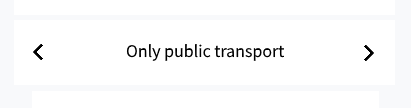
\includegraphics[width=0.5\textwidth]{Images/TravelAlternatives.png}}%
\end{figure}
\\The function checkTravelAlternative reads the selected alternative and computes the travel with the inserted TravelType.
\\View more detailed these steps:
\begin{enumerate}
	\item There is a control on a travel type selected from the user and there are two possible cases:
		\begin{enumerate}
			\item 'only-own-car' or 'only-public-transport' or 'green:
				when one these travel type is selected, it is created a new travel alternative based on related travel mode (driving for only-own-car, transit for only-public-transport and bicycling for green).
			\item 'faster' or 'cheaper':  in this case, it is created a set that contains all possible travel computable.
		\end{enumerate}
	\item Then it is selected the travel alternative:
		\begin{enumerate}
			\item In case of cheaper or faster travel, it is necessary to find among all computed travels the cheaper or the faster.
			\item In other cases, return the only one alternative computed.
		\end{enumerate}
\end{enumerate}

\begin{algorithmic}

	\Function {checkTravelAlternative}{travel, travelType}
		
		\If {travelType is 'only-own-car'}
			\State 	compute driving travel alternative
		\ElsIf {travelType is 'only-public-transport'}
			\State 	compute transit travel alternative
		\ElsIf {travelType is 'green'}
			\State 	compute bicycling travel alternative
		\ElsIf {travelType is 'faster' or travelType is 'cheaper'}
			\State 	compute a set of differents travel alternatives
		\EndIf
		\If {travel alternative exists}
			\If {travelType is 'faster'} 
				\State find faster travel in the computed set and return it
			\EndIf
			\If travelType is 'cheaper'
				\State find cheaper travel in the computed set and return it
			\EndIf
			\State \Return the travel alternative found
		\EndIf
	\EndFunction
\end{algorithmic}

\subsubsection{Check movement alternative}
When the user views a movement details and clicks on a "means icon" from the bar, the system calls this function that read the movement type selected and computed the relative movement.	
\\ If the user selects 'car-sharing' or 'bike-sharing' it is added a new movement to reach the car or bike.

\begin{algorithmic}
	\Function {checkMovementAlternative}{movement, movementType}
		\If {movementType is 'car'}
			\State compute driving movement
		\ElsIf {movementType is 'walk'}
			\State compute walking movement
		\ElsIf {movementType is 'public-transport'}
			\State compute transit movement
		\ElsIf {movementType is 'bike'}
			\State compute bicycling movement
		\ElsIf {movementType is 'car-sharing'}
			\State compute walking movement to reach the car
			\State add a further driving movement
		\ElsIf {movementType is 'bike-sharing'}
			\State compute walking movement to reach the bike
			\State add a further bicycling movement
		\EndIf
	
		\If{computed movement exists}
			\State \Return movement alternative
		\EndIf
	\EndFunction

\end{algorithmic}


	
	%------------------------------------------------------------------------------------------------------------------------------------------------
	\clearpage
	{\color{Blue}{\section{User interface design}}}
	\label{sect:UserInterfaceDesign}
	\subsection{Registration/Login}

\begin{figure}[!h]
	\centering
	\makebox[\textwidth][c]{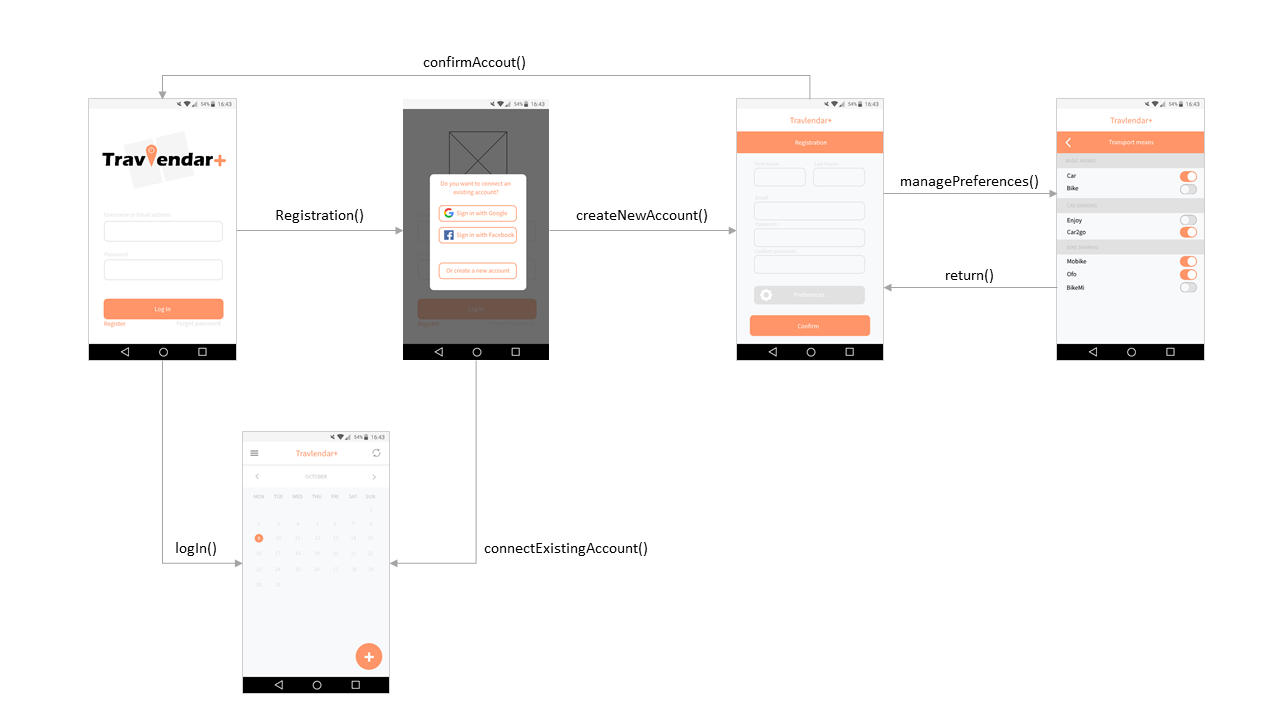
\includegraphics[width=1.4\textwidth]{Images/UI/LogIn.PNG}}%
	\caption{User Interface: registration and login}
\end{figure}
\clearpage

\subsection{Calendar views}

\begin{figure}[!h]
	\centering
	\makebox[\textwidth][c]{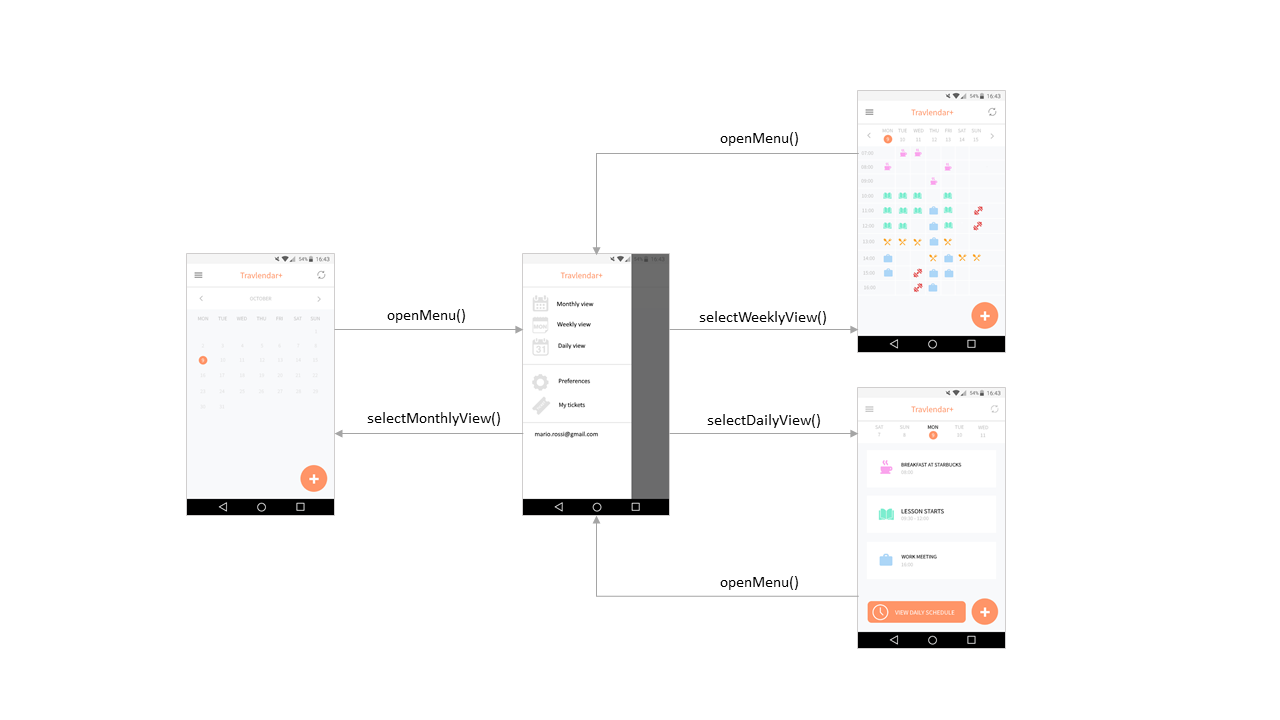
\includegraphics[width=1.4\textwidth]{Images/UI/Views.PNG}}%
	\caption{User Interface: calendar views and menu}
\end{figure}
\clearpage

\subsection{Create new appointment}

\begin{figure}[!h]
	\centering
	\makebox[\textwidth][c]{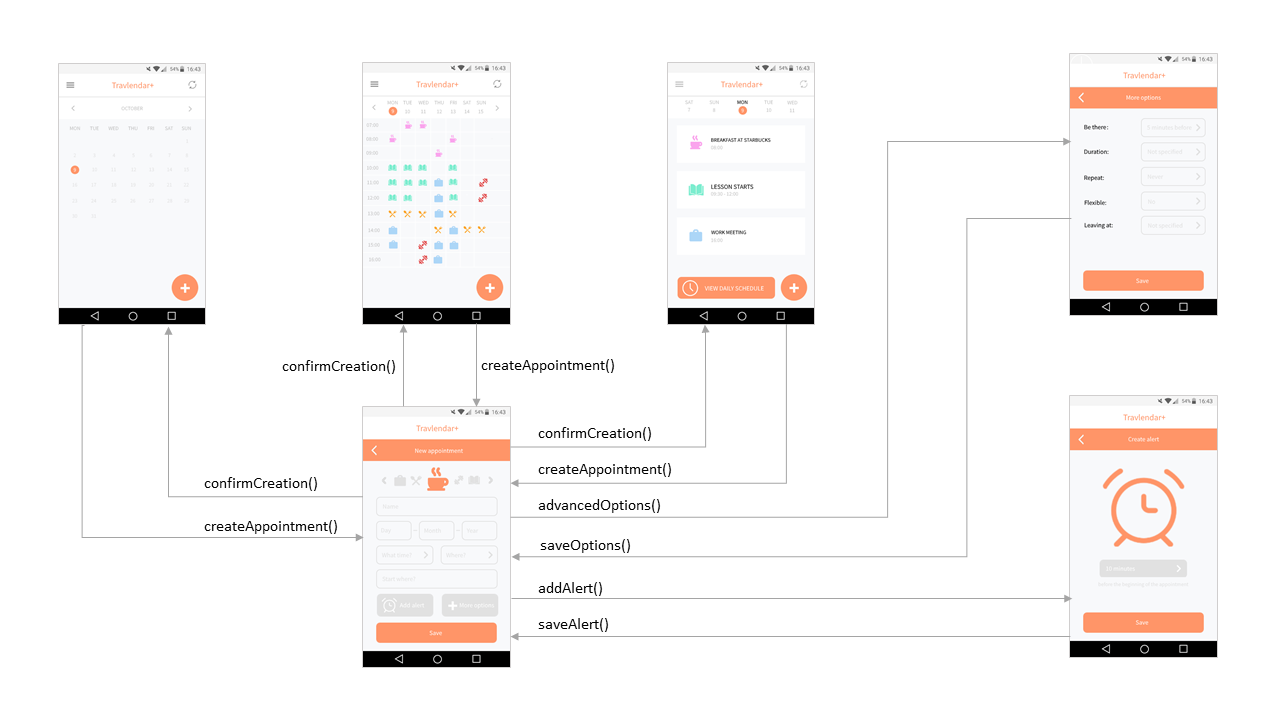
\includegraphics[width=1.4\textwidth]{Images/UI/New.PNG}}%
	\caption{User Interface: creation of new appointment}
\end{figure}
\clearpage

\subsection{Edit existing appointment}

\begin{figure}[!h]
	\centering
	\makebox[\textwidth][c]{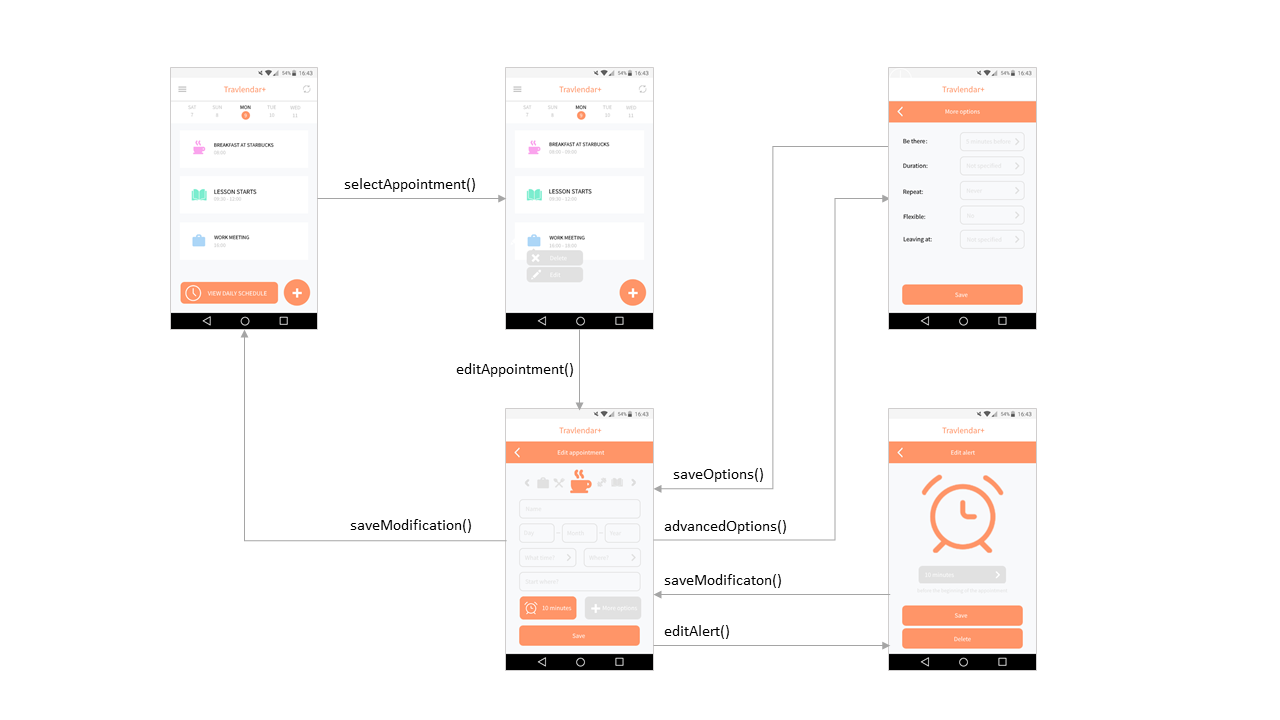
\includegraphics[width=1.4\textwidth]{Images/UI/Edit.PNG}}%
	\caption{User Interface: edit of an existing appointment}
\end{figure}
\clearpage

\subsection{manage preferences}
\begin{figure}[!h]
	\centering
	\makebox[\textwidth][c]{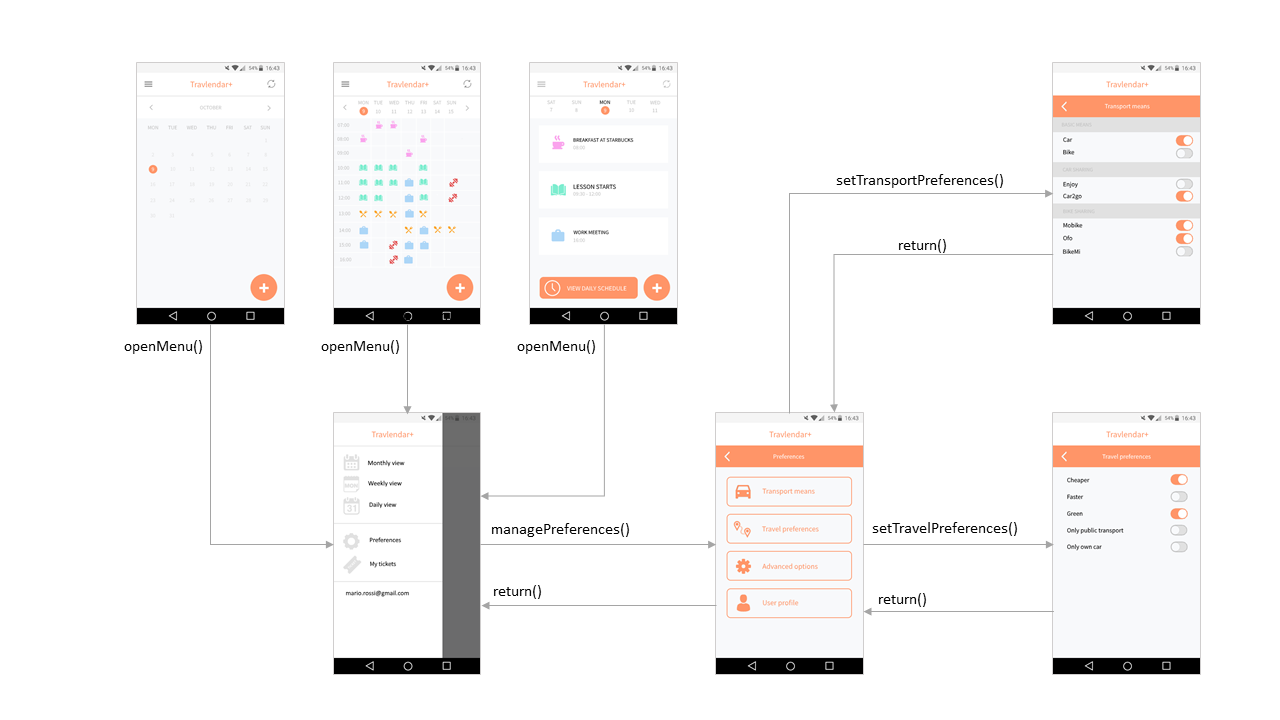
\includegraphics[width=1.4\textwidth]{Images/UI/Preferences.PNG}}%
	\caption{User Interface: manage preferences}
\end{figure}
\clearpage

\subsection{View daily schedule and travel/movement details}

\begin{figure}[!h]
	\centering
	\makebox[\textwidth][c]{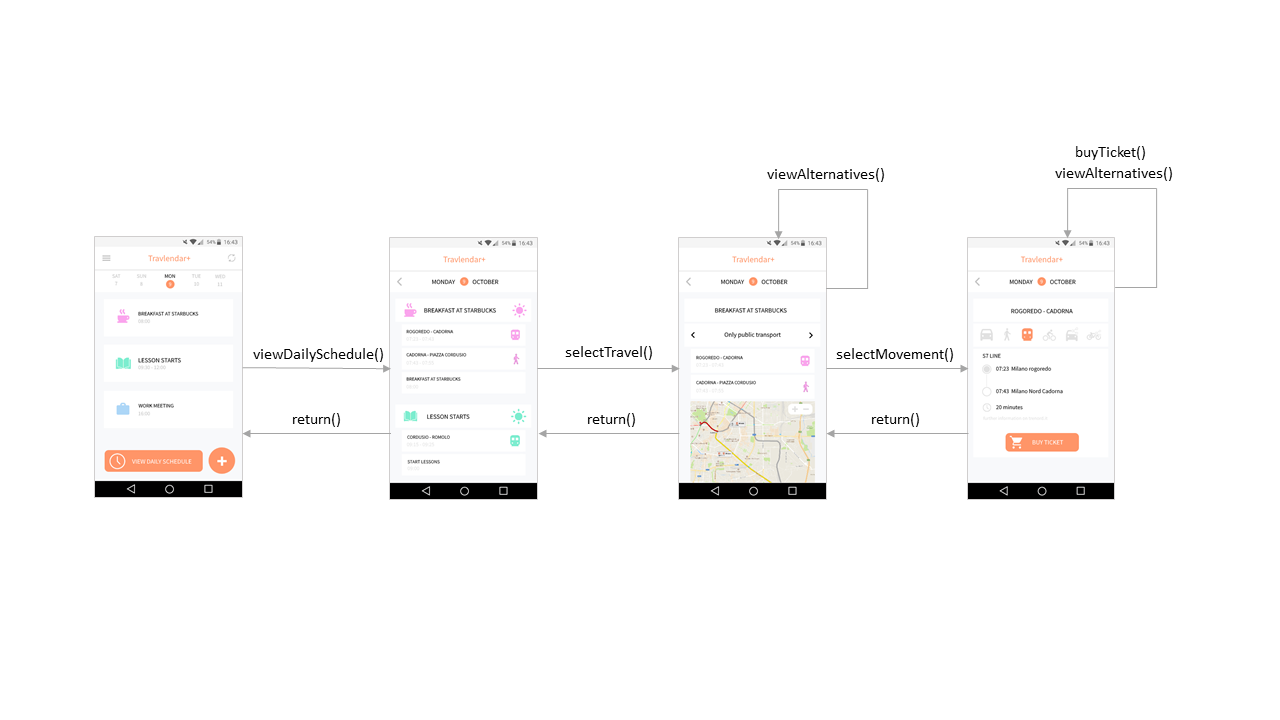
\includegraphics[width=1.4\textwidth]{Images/UI/Schedule.PNG}}%
	\caption{User Interface: daily schedule and travel/movement details}
\end{figure}
\clearpage

\subsection{Buy and view tickets}

\begin{figure}[!h]
	\centering
	\makebox[\textwidth][c]{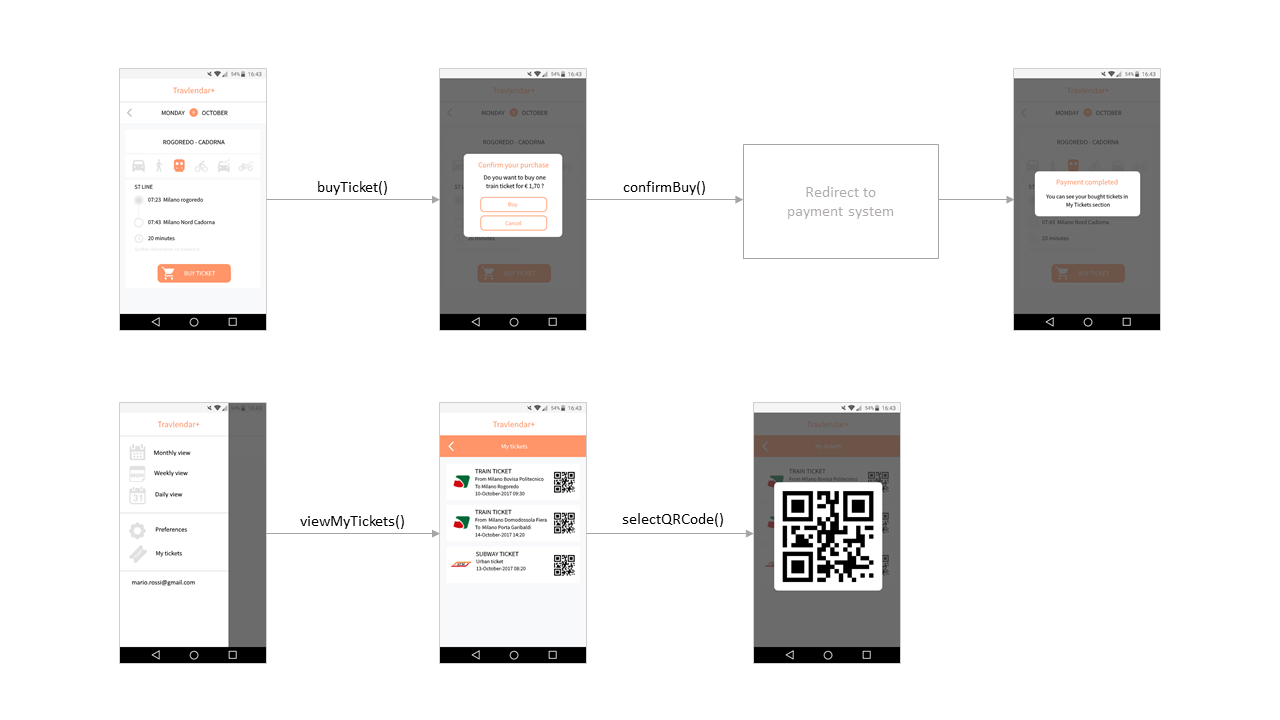
\includegraphics[width=1.4\textwidth]{Images/UI/Ticket.PNG}}%
	\caption{User Interface: buy ticket and 'My tickets' section}
\end{figure}
\clearpage
	
	%------------------------------------------------------------------------------------------------------------------------------------------------
	\clearpage
	{\color{Blue}{\section{Requirements traceability}}}
	\label{sect:RequirementsTraceability}
	\begin{itemize}
	\item \textbf{[R1] The user must be logged into the system to access application features.}\\
As explained in the IITP part, there is dependency between Travel and Appointment Manager and Account Manager: the account managing infrastructure is created first and travel/appointment data are acquired from the database.

\item \textbf{[R2] The user must be able to choose the option of creating a new appointment.}\\
Appointment Manager implements the functionality createAppointment(). See section~\ref{subsec:newAppointment}: Create new appointment.

\item \textbf{[R3] The user must be able to choose the option of editing a selected appointment.}\\
Appointment Manager implements the functionality editAppointment(). See section~\ref{subsec:editAppointment}: Edit existing appointment.

\item \textbf{[R4] The user must be able to choose the option of deleting a selected appointment.}\\
Appointment Manager implements the functionality deleteAppointment().

\item \textbf{[R5] The system must be able to provide the user with an overview of his calendar and the user
must be able to view all appointments fixed in a certain period.}\\
The system gets information about all the created appointment from the database and display them to with the interfaces described in the User Interfaces section of this document.

\item \textbf{[R6] The user must be able to select a chosen day from the overview of his calendar.}\\
The system keeps track of the different dates (see Class Diagram: Date class) and offers the daily calendar option of display. See section~\ref{subsec:view}: Calendar views.

\item \textbf{[R7] The user must be able to select a specific appointment in his calendar.}\\
Account Manager loads the information about the different appointments (see Class Diagram: Appointment class). See section~\ref{subsec:editAppointment}: Editing existing appointment to see the correspondent user interfaces.

\item \textbf{[R8] The system must ask the user to provide all information needed for the creation of a new
appointment, such as place and time of start and overall duration.}\\
This requirement is covered by the createAppointment() functionality of Appointment Manager. See section~\ref{subsec:newAppointment}: Create new appointment.

\item \textbf{[R9] The system must check if the information provided by the user are correct.}\\
Functionalities covered during phases of creation/editing. See Sequence diagrams on section 5.2 of RASD document.

\item \textbf{[R10] The system must check if an appointment overlaps with other events and must eventually
notify it to the user.}\\
See section~\ref{subsec:algOverlap}: Check overlap algorithm.

\item \textbf{[R11] The system must give the user access to all details of a selected appointment and the user
must be allowed to edit the information needed.}\\
Account Manager loads the information about the different appointments (see Class Diagram: Appointment class) and display them to the user. It also implements the functionality editAppointment(). See section~\ref{subsec:editAppointment}: Editing existing appointment to see user interfaces.

\item \textbf{[R12] The user must be able to set advanced information for a created appointment.}\\
See advancedOptions() in section~\ref{subsec:newAppointment}: Create new appointment.

\item \textbf{[R13] The user must be able to set an appointment as flexible, specifying the interval of time.}\\
Functionality of Appointment Manager. See advancedOptions() in section~\ref{subsec:newAppointment}: Create new appointment and the Flexible Appointment class in the Class Diagram.

\item \textbf{[R14] The user must be able to set an appointment as repeatable, specifying the desired days.}\\
Functionality of Appointment Manager. See advancedOptions() in section~\ref{subsec:newAppointment}: Create new appointment.

\item \textbf{[R15] The system must schedule any flexible or repeatable appointment in the correct way, avoiding overlapping with other appointments.}\\
The system is provided with algorithm for overlapping checking and flexible appointments scheduling. See section~\ref{subsec:algorithm} for further info.

\item \textbf{[R16] The appointment intended to be modified must have been previously successfully created
and not already deleted.}\\
The process of editing appointments is made by Appointment Manager and works only with existing appointments in the database. A process is stored in the database only at the creation and removed during the deletion. See section~\ref{subsec:runtimeView}: Runtime view.

\item \textbf{[R17] The user must confirm the creation of the new appointment.}\\
createAppointment() functionality of Appointment Manager. See confirmCreation() in section~\ref{subsec:newAppointment}: Create new appointment.

\item \textbf{[R18] The user must confirm any appointment modification.}\\
editAppointment() functionality of Appointment Manager. See saveModification() in section~\ref{subsec:newAppointment}: Create new appointment.

\item \textbf{[R19] The system must save the user modifications in memory and the calendar must be updated.}\\
Appointment Manager interacts with the DBMS: after any modification, the database is updated. See section 2.4: Runtime view.

\item \textbf{[R20] The system must remove a deleted appointment from the memory and delete every alert
related to it.}
Appointment Manager interacts with the DBMS: after any modification, the database is updated.
This functionality is implemented by deleteAppointment().

\item \textbf{[R21] The user must be able to switch between different possible calendar, such as daily calendar, weekly calendar and monthly calendar.}\\
See section~\ref{subsec:view}: Calendar view.

\item \textbf{[R22] The system must be able to provide information about the scheduled travels for a chosen
day, showing the transport means and the estimated time required from each travel.}\\
User can recall the function viewDailySchedule() from his application, and Travel Manager takes care of provide all the information in detail. See section~\ref{subsec:runtimeView}: Runtime view.

\item \textbf{[R23] The system must choose the best option between the possible travel alternatives according
to the preferences expressed in the user profile settings and the information about external weather.}\\
This requirement is covered by the computeTravel() and loadPreferences() functionality of Travel Manager. See section~\ref{subsec:algComputeTravel}: Compute travel for further info on the algorithm.

\item \textbf{[R24] The user must be able to select a specific travel in his daily schedule.}\\
See selectTravel() in section~\ref{subsec:dailySchedule}: View daily schedule and travel/movement details.

\item \textbf{[R25] The system must provide detailed information about the travels selected by the user, such
as the trace route on the map and the weather conditions.}\\
This requirement is covered by the computeTravel() functionality of Travel Manager. More specifically, see section~\ref{subsec:runtimeView} for runtime view and section~\ref{subsec:algComputeTravel}: Compute travel for further info on the algorithm.

\item \textbf{[R26] The system must provide the user with an overview of the possible travel alternatives for the chosen travel, specifying all details for each one.}\\
Travel Manager functionalities. see section~\ref{subsec:algTravelAlternative}: Check travel alternative for further info on the algorithm and viewAlternatives() in section~\ref{subsec:dailySchedule}: View daily schedule and travel/movement details for user interfaces.

\item \textbf{[R27] The user must be able to filter the travel alternatives furnished.}\\
Travel Manager functionalities. see section~\ref{subsec:algTravelAlternative}: Check travel alternative for further info on the algorithm.

\item \textbf{[R28] The user must be able to choose a favorite travel option different from the displayed default one.}\\
Travel Manager functionalities. See section~\ref{subsec:algTravelAlternative}: Check travel alternatives for further info on the algorithm.

\item \textbf{[R29] The user must be able to select a specific movement in a travel.}\\
See selectMovement() in section~\ref{subsec:dailySchedule}: View daily schedule and travel/movement details.

\item \textbf{[R30] The system must provide detailed information about the movements selected by the user,
such as the specific trace route on the map and the price of the ticket.}\\
Travel Manager functionalities. All information are provided by the external APIs and collected by the system as explained in section~\ref{subsec:runtimeView}. See section~\ref{subsec:dailySchedule}: View daily schedule and travel/movement details for user interfaces.

\item \textbf{[R31] The user must be able to choose an alternative transport mean for a selected movement, if
there are any.}\\
Travel Manager functionalities. See section~\ref{subsec:algMovementAlternative}: Check movement alternative for further info on the algorithm.

\item \textbf{[R32] The system must update the daily schedule according to the travel option chosen by the user and the user must be able to see the new updated schedule.}\\
Travel Manager functionality. The user can choose a travel alternative (see section~\ref{subsec:algTravelAlternative}: Check travel alternative for info on the algorithm) and Travel Manager updates info.

\item \textbf{[R33] The system must give to the user the possibility of buying the ticket for the selected travel.}\\
This requirement is covered by Ticket Manager functionalities. See section~\ref{subsec:dailySchedule}: Component interfaces for full functionalities overview.

\item \textbf{[R34] The system must save a copy of the bought tickets.}\\
Tickets manager interacts with DMBS to store tickets data after the purchase. See section~\ref{subsec:runtimeView} for runtime views.

\item \textbf{[R35] The user must be able to access to a ticket page from the home page.}\\
Bought tickets are saved in the database during the purchase process (see section~\ref{subsec:runtimeView} for runtime view) and the user can access them by clicking on “My tickets) on the side panel menu. See section~\ref{subsec:ticket}: Buy and view tickets for user interfaces.

\item \textbf{[R36] The system must provide a list of all the bought tickets and the user must be able to select
and view a specific one.}\\
This requirement is covered by the viewTickets() functionality of Travel Manager. See section~\ref{subsec:ticket}: Buy and view tickets for user interfaces.

\item \textbf{[R37] The user must be able to access the preferences panel of his account.}\\
Account Manager functionality. See section~\ref{subsec:preferences}: Manage preferences for user interfaces.

\item \textbf{[R38] The system must give the user the possibility of setting various preferences, such as owned
and preferred travel means, address of Home and other general travel preferences.}\\
Account Manager functionality. See section~\ref{subsec:preferences}: Manage preferences for user interfaces.

\item \textbf{[R39] The user must be able to edit the provided preferences when needed.}\\
The preferences panel is always accessible from the home page (See section~\ref{subsec:preferences}: Manage preferences for user interfaces). Account Manager interacts with DBMS, so any modification will be update in the database.

\item \textbf{[R40] The system must give the user the possibility of adding an alert to an appointment while it is being created or modified.}\\
Functionality of Appointment Manager. See section 5.2.3 and 5.2.4 or RASD document: Appointment creation and Appointment editing for info on Sequence diagrams and sections~\ref{subsec:newAppointment}/~\ref{subsec:editAppointment} of this document for user interfaces

\item \textbf{[R41] The user must be able to choose a desired interval of time for the warning alert.}\\
Functionality of Appointment Manager. See section 5.2.6 of RASD document: Alert editing for info on Sequence diagrams and sections~\ref{subsec:newAppointment}/~\ref{subsec:editAppointment} of this document for user interfaces.

\item \textbf{[R42] The user must confirm the alert creation and the system must save the insertion in the memory.}\\
Appointment manager interacts with DBMS to store information in the system memory. See section 5.2.6 of RASD document: Alert editing for info on Sequence diagrams and sections~\ref{subsec:newAppointment}/~\ref{subsec:editAppointment} of this document for user interfaces.

\item \textbf{[R43] The user must be able to modify or remove the inserted alert when needed.}\\
Appointment manager functionalities are always accessible by the user through the correspondent interfaces.

\item \textbf{[R44] In case of any alert modification made by the user, the user must confirm the modification
and the system must save all changes.}\\
Appointment manager interacts with DBMS and updates data after any modification. See section 5.2.6 of RASD document: Alert editing for info on Sequence diagrams and sections~\ref{subsec:newAppointment}/~\ref{subsec:editAppointment} of this document for user interfaces.
\end{itemize}

	
	%------------------------------------------------------------------------------------------------------------------------------------------------
	\clearpage
	{\color{Blue}{\section{Implementation, integration and test plan}}}
	\label{sect:TestPlan}
	\subsection{Overview}

As explained in the RASD and DD documents, the system requires the following components to be fully developed and working:
\begin{itemize}
	\item \textbf{Travlendar+ mobile application, working on Android v 4.0.3 and later;}
	\item \textbf{JBoss 7.0.1 Java Server, running the Travlendar+ application services;}
	\item \textbf{MySQL 5.7.19 DBMS for users data managing;}
\end{itemize}
Furthermore, the Travlendar+ application services component is composed by the following subsystems, which must be developed and correctly integrated:
\begin{itemize}
	\item \textbf{Appointment manager}, which makes use of Calendar APIs and requires DBMS connection;
	\item \textbf{Travel manager}, which implements Weather and Maps APIs;
	\item \textbf{Account manager},
	\item \textbf{Tickets manager},
\end{itemize}
Finally, the following connection must be implemented and full working:
\begin{itemize}
	\item \textbf{Remote Method Invocation} connection between client and application server, using JRMP protocol;
	\item \textbf{JDBC} connection between application server and DBMS.
\end{itemize}

\subsection{Strategy}
In order to guarantee observability and efficacy, the testing strategy follows an incremental integration logic. The chosen approach is bottom-up: this choice allows us to gradually build the system and continuously provide feedbacks as soon as the single parts are finished. Our goal is to first develop sub-component that are able to work independently and do not require connections with other parts of the systems. Then, once that all sub-components are fully developed and tested, we plan to proceed in connecting them and fulfill the dependencies to implement gradually the main super-component functions. Final part of the integration will require the main component to be full working and tested, and consists in testing the correct working of connections between main-components. 

\subsection{Dependecies}
The interaction with DBMS is essential for the correct working of all the four main components of the Application services. Plus, Appointment Manager requires Account Manager to be implemented to ensure the correctness of the links between different accounts and relative calendars:

\begin{figure}[H]
	\centering
	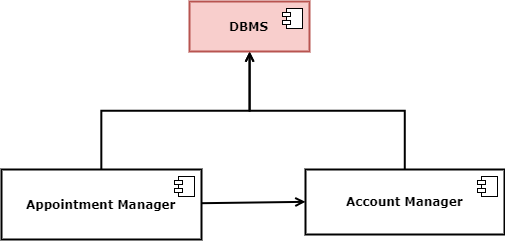
\includegraphics[width=0.9\textwidth]{Images/Test/1.png}%
\end{figure}

In order to work properly, Travel Manager makes use of different external APIs such as Maps APIs, Weather APIs and different APIs from car sharing and bike sharing services. The correct functionality of these interfaces must be checked before proceeding in developing the component. In addition, Travel Manager requires an integration with Appointment Manager to acquire data relative to the different locations of the appointments.

\begin{figure}[H]
	\centering
	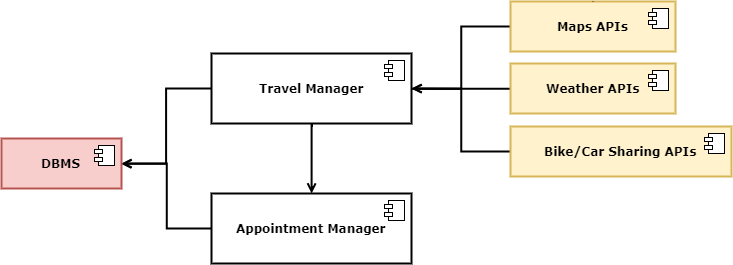
\includegraphics[width=1\textwidth]{Images/Test/2.png}%
\end{figure}

Finally, Tickets Manager strictly depends on the correct working of the APIs of the chosen ticket provider to pay and acquire travel tickets. It also requires Travel Manager to work properly, because the user can accesstickets functionalities only after selecting a movement from the daily schedule. 

\begin{figure}[H]
	\centering
	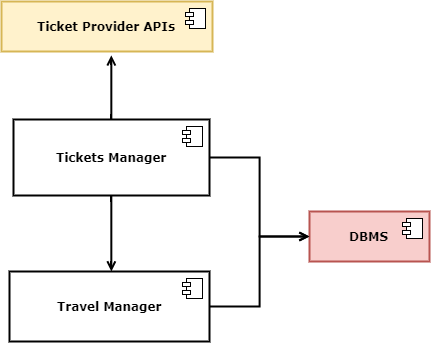
\includegraphics[width=0.8\textwidth]{Images/Test/3.png}%
\end{figure}

Given the previous information, an appropriate plan of integration and testing could be the following one:\\
\textbf{Week 27/11/17 – 4/12/17:}
\begin{itemize}
	\item DBMS: build a simple Java application that interacts with MySQL 5.7.19 Database Manage System by JDBC and correctly store and manage data from a small database.
	\item ACCOUNT MANAGER: expand the application, allowing different users to register and insert personal info. 
	\item MAPS APIs: testing APIs with small example applications to ensure correct working.
	\item WEATHER APIs: testing APIs with small example applications to ensure correct working.
\end{itemize}
\textbf{Week 4/12/17 – 11/12/17:}
\begin{itemize}
	\item CAR/BIKE SHARING APIs: testing APIs with small example applications to ensure correct working.
	\item ACCOUNT MANAGER: fully development and testing of all component functionalities: allow multiple users to register and login, manage personal data and connect existing Facebook/Google account.
	\item APPOINTMENT MANAGER: expand the application by giving the user the possibility of creating, editing and delete simple appointments (no alert/advanced option). Test the correct storage in the database and the correct integration with Account Manager.
	\item start working on network platform: develop a small application that makes use of RMI technology to invoke methods on an example application running on JBoss 7.0.1 Java Server.
\end{itemize}
\textbf{Week 11/12/17 – 18/12/17:}
\begin{itemize}
	\item APPOINTMENT MANAGER: fully development and testing of all component functionalities: allow the user to add advanced options to the different appointments. Test full integration with Account Manager.
	\item TRAVEL MANAGER: integrate use of Maps/Weather/Car\&Bike Sharing APIs with data provided by Appointment Manager to compute travels for each appointment. Testing of the functionalities.
	\item TICKET PROVIDER APIs: testing APIs with small example applications to ensure correct working.
	\item Export the application on JBoss 7.0.1 Java Server, testing of RMI methods to access the application features from remote.
\end{itemize}
\textbf{Week 18/12/17 – 8/1/18:}
\begin{itemize}
	\item TRAVEL MANAGER: fully development and testing of all component functionalities: the application accesses correctly appointment and user data to compute travels. Test complete integration with Appointment Manager.
	\item TICKET MANAGER: expand the application by adding functionalities for tickets purchase using the tested APIs. Test integration with Travel Manager.
\end{itemize}
\textbf{Week 8/1/18– 18/1/18:}
\begin{itemize}
	\item General testing of full application functionalities.
\end{itemize}
	
	%------------------------------------------------------------------------------------------------------------------------------------------------
	\clearpage
	{\color{Blue}{\section{Effort spent}}}
	\label{sect:EffortSpent}
	
\subsubsection{Andrea Mafessoni}

\begin{table}[h!]
	\begin{tabular}{lcccc}
		\toprule
		\textbf{Task name} & \textbf{Start date} & \textbf{End date} & \textbf{Hours(h)} & \textbf{Day} \\
		\midrule
		\textbf{RASD} & \textbf{02/11/2017} & \textbf{25/11/2017} & \textbf{24.5} & \\
		Brainstorming and general overview & 02/11/2017 & 12/11/2017 & 5 & 11 \\
		2. Architectural Design (Deployment view) & 12/11/2017 & 14/11/2017 & 4 & 3 \\
		5. Requirements Traceability & 22/11/2017 & 24/11/2017 & 3.5 & 3 \\
		2. Architectural Design (Component view) & 21/11/2017 & 23/11/2017 & 6 & 3 \\
		6. Implementation, integration and test plan & 16/11/2017 & 21/11/2017 & 4 & 6 \\
		\bottomrule
		Final revision & 20/11/2017 & 25/11/2017 & 3 & 6 \\
	\end{tabular}
\end{table}

\begin{figure}[!h]
	\centering
	\makebox[\textwidth][c]{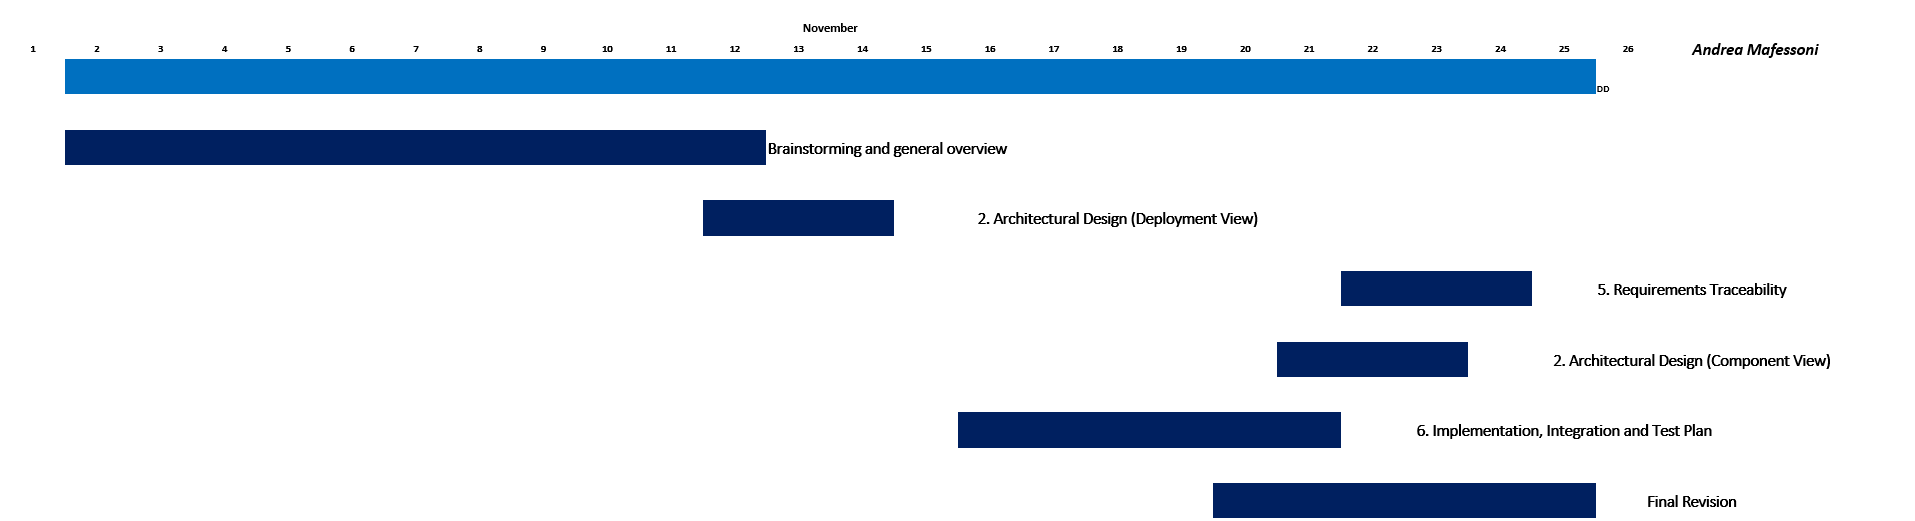
\includegraphics[width=1.2\textwidth]{Images/Gantt/andreaMafessoni.png}}%
	\caption{Gantt diagram Mafessoni}
\end{figure}
\clearpage

\subsubsection{Andrea Mazzeo}

\begin{table}[h!]
	\begin{tabular}{lcccc}
		\toprule
		\textbf{Task name} & \textbf{Start date} & \textbf{End date} & \textbf{Hours(h)} & \textbf{Day} \\
		\midrule
		\textbf{RASD} & \textbf{02/11/2017} & \textbf{25/11/2017} & \textbf{23.5} &  \\
		Brainstorming and general overview & 02/11/2017 & 12/11/2017 & 5 & 11 \\
		3. Algorithm design & 04/11/2017 & 9/11/2017 & 6 & 6 \\
		4. User interface Design & 06/11/2017 & 14/11/2017 & 4 & 10 \\
		1. Introduction & 23/11/2017 & 24/11/2017 & 1 & 2 \\
		Latex & 16/11/2017 & 25/11/2017 & 4.5 & 10 \\
		\bottomrule
		Final revision & 20/11/2017 & 25/11/2017 & 3 & 6 \\
	\end{tabular}
\end{table}

\begin{figure}[!h]
	\centering
	\makebox[\textwidth][c]{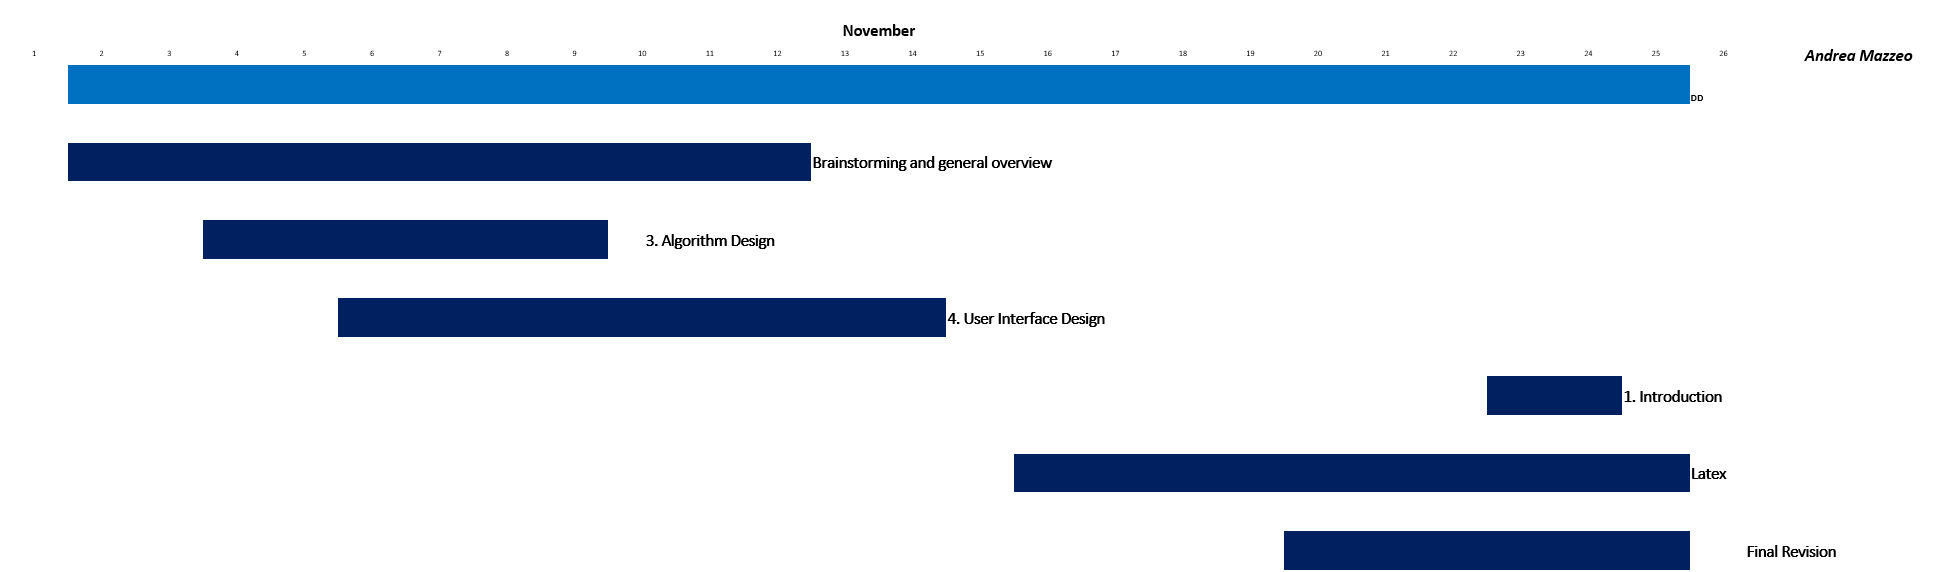
\includegraphics[width=1.2\textwidth]{Images/Gantt/andreaMazzeo.png}}%
	\caption{Gantt diagram Mazzeo}
\end{figure}
\clearpage

\subsubsection{Daniele Moltisanti}

\begin{table}[h!]
	\begin{tabular}{lcccc}
		\toprule
		\textbf{Task name} & \textbf{Start date} & \textbf{End date} & \textbf{Hours(h)} & \textbf{Day} \\
		\midrule
		\textbf{Design document} & \textbf{02/11/2017} & \textbf{25/11/2017} & \textbf{21} &  \\
		Brainstorming and general overview & 02/11/2017 & 12/11/2017 & 5 & 11 \\
		2. Architectural Design (Overview) & 05/11/2017 & 06/11/2017 & 2 & 2 \\
		2. Architectural Design (Component view) & 09/11/2017 & 12/11/2017 & 3.5 & 4 \\
		2. Architectural Design (Runtime view) & 15/11/2017 & 22/11/2017 & 4.5 & 8 \\
		2. Architectural Design (Component interface) & 16/11/2017 & 24/11/2017 & 2 & 9 \\
		2. Architectural Design (Architectural style and pattern) & 14/11/2017 & 15/11/2017 & 1 & 2 \\
		\bottomrule
		Final revision & 20/11/2017 & 25/11/2017 & 3 & 6 \\
	\end{tabular}
\end{table}

\begin{figure}[!h]
	\centering
	\makebox[\textwidth][c]{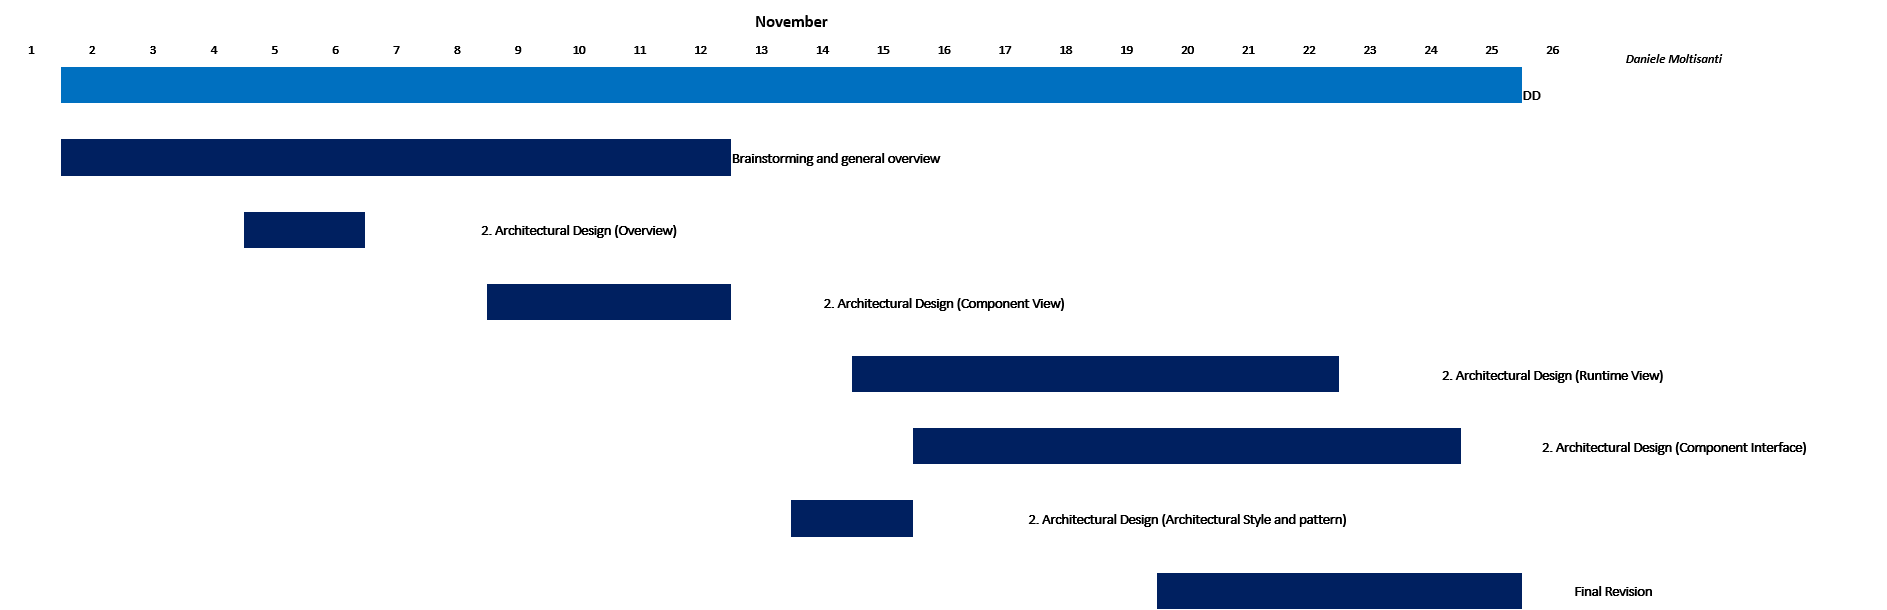
\includegraphics[width=1.2\textwidth]{Images/Gantt/danieleMoltisanti.png}}%
	\caption{Gantt diagram Moltisanti}
\end{figure}
\clearpage
	%------------------------------------------------------------------------------------------------------------------------------------------------
	
	
	
	
\end{document}
